\section{Architektur}\label{sec:architecure}

\captionsetup[table]{name=Abbildung}
\renewcommand\thetable{8}
\begin{table*}[!ht]
	\centering
	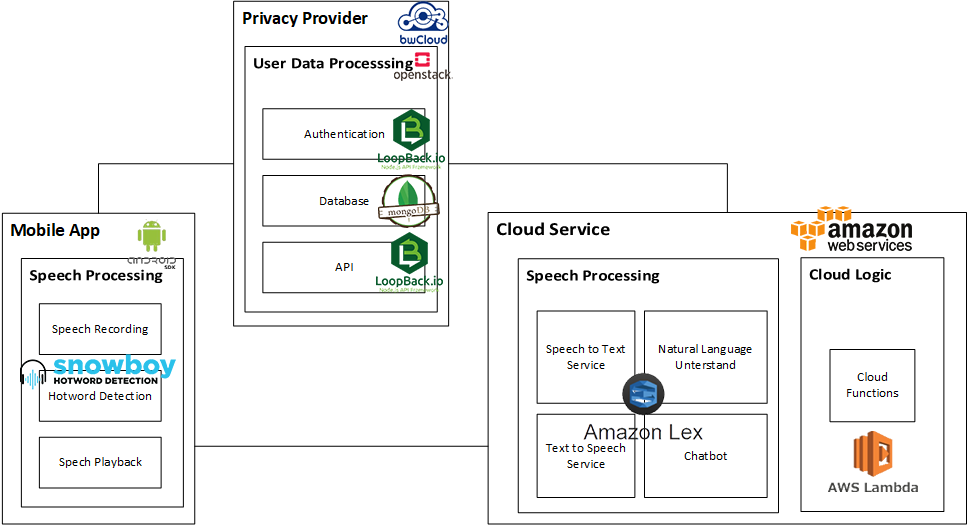
\includegraphics[width=1\linewidth]{Picture/Architektur}
	\caption[Archtiktur Übersicht]{Archtiktur Übersicht}
	\label{fig:architecure}
\end{table*}

Das im letzten Kapitel vorgestellte Konzept wird anhand der in Abbildung \ref{fig:architecure} aufgezeigten Architektur und Technologien umgesetzt. Dabei werden drei Komponenten zur Umsetzung benötigt:
 
\begin{itemize}
    \item Mobile App: Die Mobile App dient als Schnittstelle zum Nutzer. Der Nutzer kann über die App Spracheingaben tätigen sowie sein Profil und Privatsphäre konfigurieren.
    \item Cloud Services: Diese Komponente übernimmt die Sprachverarbeitung und die Erzeugung einer Ausgabe an den Nutzer. Dabei wird zur Erzeugung einer Antwort auf den Privacy Provider zugegriffen.
    \item Privacy Provider: Der Privacy Provider ist das Kernstück, wodurch dem Nutzer mehr Privatsphäre gewährleistet wird. Der genaue Aufbau sowie die Technologieauswahl wird im Folgenden beschrieben. 
\end{itemize}

Für die Kommunikation zwischen mobiler App und der Cloud Services mit dem Privacy Provider wurde eine RESTful \ac{api} ausgewählt. Die \ac{api} basiert auf der RESTful-Technologie, einem Architektur- und Kommunikationsmuster, das häufig bei der Entwicklung von Webdiensten zum Einsatz kommt. Mittels HTTP-Anforderungen wie z.B. GET, PUT-, POST- und DELETE- können Daten ausgetauscht und gespeichert werden \cite{restful-api}. Für die Umsetzung der „Speech Triggered Mobility Support and Privacy“ Anwendung, wurden virtuelle Maschinen, gehostet bei bwCloud, erstellt. Die bwCloud stellt mit Hilfe von OpenStack, \ac{iaas} für Forschung und Lehre in Baden-Württemberg bereit. Sie ermöglicht den Aufbau und Betrieb einer standortübergreifenden Infrastruktur zur Bereitstellung von Computer-Ressourcen \cite{bw-cloud}. Bei Bedarf kann eine bestehende virtuelle Maschine um zusätzliche Ressource erweitert werden, was die Skalierbarkeit des Projektes für zukünftige Anforderungen oder Erweiterungen vereinfacht. Die virtuelle Maschine wird mit Ubuntu Server 18.04.1 LTS betrieben. Mit Hilfe eines 2048Bit RSA Schlüssels kann Verbindung zur virtuellen Maschine hergestellt werden. Für die Umsetzung der REST \ac{api} wurden verschiedene Frameworks betrachtet. 

Loopback ist ein stark erweiterbares, Open-Source Node.js Framework, welches die Entwicklung schneller dynamischer End-to-End REST \ac{api}s ermöglicht. Loopback zeichnet sich durch eine große Community, ausgezeichnete Dokumentation, Vielzahl an Support Möglichkeiten (IBM, StrongLoop) sowie einem breitem Einsatzgebiet aus. Des Weiteren wird es unter anderem auch für kommerzielle Einsatzgebiete, wie z.B. bei der Bank of America, Symantec und der amerikanischen Energiebehörde (Department of Energy) eingesetzt \cite{loopback}.

Loopback ermöglicht es, REST \ac{api}s über ein Command Line Interface Wizard zu erstellen. Es können dynamische Modelle, basierend auf dem gewünschten Datenschema, erstellt werden. Ein weiterer ausschlaggebender Punkt für die Auswahl von Loopback, ist die Unterstützung von Beziehungen unter den erstellten Modellen und der automatischen Erstellung zugehöriger relationaler REST-Endpunkte. Das Framework ermöglicht die Umsetzung einfacher Authentifizierung und Autorisierung durch integrierte rollenbasierte Zugriffskontrollen. Eine Anmeldung von Drittanbietern und OAuth2 ist ebenfalls möglich \cite{mongodb}.

Für die Umsetzung wurde die Loopback Version 3.24.1 verwendet. Das Framework zeichnet sich durch seine Flexibilität aus. Es kann auf einem lokalen Server oder in der Cloud betrieben werden. Ein browserbasierter Explorer ermöglicht Interaktionen mit der \ac{api}. Loopback unterstützt die Anbindung von mehreren Datenspeichern. Für die Umsetzung wurde die Open Source Datenbank MongoDB ausgewählt. MongoDB ist ein verteiltes, flexibles, dokumentbasiertes Datenmodell. Daten werden in JSON-ähnlichen Dokumenten gespeichert. Dies ermöglicht eine Veränderung der Datenstruktur im Laufe der Zeit. Funktionen für Hochverfügbarkeit und Skalierung sowie geografische Verteilung sind einfach durchzuführen \cite{mongodb}. Diese Eigenschaften ermöglichen eine spätere Anpassung oder Verteilung der Infrastruktur.

